\documentclass{article}

%Hiermee zet je de taal van het document op Nederlands, zodat de spellingscontrole van LaTeX werkt. Daarnaast komen ook automatische koppen als inhoudsopgave en referenties in het Nederlands in de tekst
\usepackage[dutch]{babel}
\addto{\captionsdutch}{\renewcommand{\abstractname}{Abstract}}

%Deze packages zorgen ervoor dat jouw referenties in APA format weergegeven worden
\usepackage{hyperref}
\usepackage{natbib}
\usepackage{apalike}
\bibliographystyle{apalike}

%Hierdoor worden speciale tekens als -/'" juist weergegeven in de tekst
\usepackage[utf8]{inputenc}

%Deze commando' s zorgen dat de titel en auteur correct op de voorpagina komen
\usepackage[T1]{fontenc}
\usepackage{authblk}
\renewcommand\Affilfont{\itshape\small}

%Multicol kan gebruikt worden om een stuk tekst op te delen in twee kolommen
\usepackage{multicol}

%Onderstaande packages zorgen ervoor dat afbeeldingen gebruikt kunnen worden en dat je captions en subcaptions kan gebruiken
\usepackage{graphicx}
\usepackage{caption}
\usepackage{subcaption}
\graphicspath{ {images/} }
\usepackage{float}
\usepackage[font=small,labelfont=bf]{caption}

%Minted is handig om te gebruiken wanneer je programmeercode wil weergeven in een verslag
\usepackage{minted}

%Hier begint het document en worden de verschillende pagina 's toegevoegd en gescheiden van elkaar door page breaks
\begin{document}

\title{Titel komt hier}
\author{Jan Jansen}
\affil{1234567}

\date{\small \today}

\maketitle

%Hiermee verschijnt er een abstract
\begin{abstract}
\noindent Lorem ipsum dolor sit amet, habeo integre qualisque ex mea, ne aliquid dignissim voluptaria ius, ex his noster verterem. An viderer petentium conclusionemque eum, est libris delicatissimi interpretaris cu. Eos ea quidam tincidunt. Facer definiebas no est, quod fugit sadipscing cum ei. An doming regione eum, velit facilis sed te.

\paragraph{keywords:} Keyword1, keyword2, keyword3
\paragraph{aantal woorden:} 1234

\end{abstract}
\pagebreak

%Hiermee wordt automatisch een inhoudsopgave aangemaakt
\tableofcontents
\pagebreak

\section{Inleiding}
Lorem ipsum dolor sit amet, consectetur adipiscing elit. Quisque gravida justo eu urna suscipit posuere. Nulla euismod purus sapien, vel fermentum orci pharetra pharetra. Aenean aliquam nulla vel tellus luctus, quis efficitur neque condimentum. Sed lacinia dictum ex, ac mollis arcu consectetur sit amet. Duis pharetra risus tincidunt nisi consequat condimentum. Praesent malesuada dapibus elit at suscipit. Donec quis nisl fermentum, luctus ligula ac, interdum neque. \figurename{ \ref{genderdetect}} \citep{norman2014incremental} %Zo roep je het correcte figuur aan. 

\begin{figure}[H] %[H] zorgt ervoor dat het figuur precies op de plek komt in de tekst waar je het zet in LaTeX

    %Hier geeft je de programmeertaal
    \begin{minted}{Python} 
        from gender_detector import GenderDetector
        
        detector = GenderDetector('us')         #language
        detector.guess('Amy')                   # => 'female'
        \end{minted}
        
        %Hier geef je een titel aan het figuur
    \caption{Python gender detector.}\label{genderdetect}
    %Het label kan gebruikt worden in de lopende tekst om te refereren naar het figuur.
    
\end{figure} 
\section{Methode}
Vestibulum viverra auctor elit et sodales. Vivamus vitae molestie ipsum. Mauris vel augue eu est scelerisque tempus vitae id justo. Etiam eu dui sed lorem placerat finibus vel quis tellus. Maecenas tristique dolor lectus, vitae egestas nisi vulputate et. Pellentesque tincidunt sapien nec libero fermentum rhoncus. Aliquam porta consequat sapien sit amet fermentum. Nunc pellentesque imperdiet tellus, ac condimentum eros elementum molestie.
%Met een witregel tussen de alinea 's zal de volgende regel inspringen
Curabitur cursus finibus lectus in dignissim. Sed pellentesque, nisi in blandit iaculis, eros purus interdum leo, quis dictum purus mi a est. Nullam in magna id lacus ultrices porttitor. Curabitur finibus ipsum nec dui semper bibendum. Suspendisse bibendum ante sed feugiat dignissim. \\

%Door \\ aan het einde van een alinea zal er een witregel tussen de alinea 's komen. Om dan te voorkomen dat de tekst ook nog inspringt gebruik je het commando no indent
\noindent Vivamus nec urna lacus. Praesent at fringilla elit. Phasellus fringilla dolor id metus sodales lobortis. Pellentesque tincidunt nec magna a rhoncus. Etiam auctor pulvinar rutrum. Morbi vel nulla nisl. Etiam convallis condimentum libero et rhoncus. Ut a hendrerit erat. Vivamus vel posuere massa. Fusce aliquam purus ut fermentum sollicitudin. Ut ut accumsan diam \footnote{Dit is een footnote}. %Zo maak je een footnote aan.

\subsection{Participanten}
Lorem ipsum dolor sit amet, consectetur adipiscing elit. Quisque gravida justo eu urna suscipit posuere. Nulla euismod purus sapien, vel fermentum orci pharetra pharetra. Aenean aliquam nulla vel tellus luctus, quis efficitur neque condimentum. Sed lacinia dictum ex, ac mollis arcu consectetur sit amet. Duis pharetra risus tincidunt nisi consequat condimentum. Praesent malesuada dapibus elit at suscipit.

%Op deze manier kunnen er twee afbeeldingen naast elkaar. 
\begin{figure}[H]
    \begin{minipage}[p]{0.48\textwidth}
        \centering
        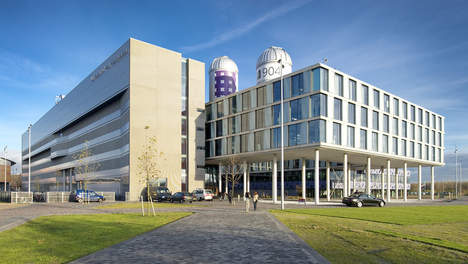
\includegraphics[width=0.95\textwidth]{SciencePark.jpg}
    \end{minipage}
    \begin{minipage}[p]{0.48\textwidth}
        \centering
        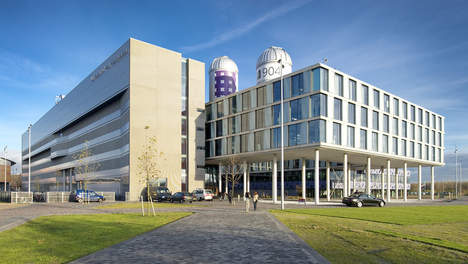
\includegraphics[width=0.95\textwidth]{SciencePark.jpg}
    \end{minipage}
    \caption{Science Park}
\end{figure}

%Zo gebruik je een losse afbeelding.
\begin{figure}[H]
    \centering
        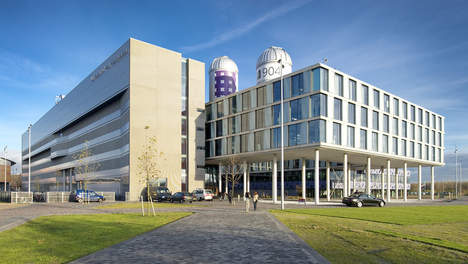
\includegraphics[width=0.7\textwidth]{SciencePark.jpg}
        \caption{Science Park}
        \centering
\end{figure}


\subsection{Procedure}
%Hierdoor wordt er een lijst aangemaakt, verdeeld over twee kolommen
\begin{itemize}
\begin{multicols}{2} %Hier geef je het aantal kolommen aan
    \item{item 1}
    \item{item 2}
    \item{item 3}
    \item{item 4}
    \item{item 5}
    \item{item 6}
\end{multicols}
\end{itemize}

\subsection{Analyse}
%Ook de tekst kan in twee kolommen gezet worden
\begin{multicols}{2}
Donec quis nisl fermentum, luctus ligula ac, interdum neque. Praesent a justo sit amet nisl aliquet consectetur nec et ipsum. Curabitur porttitor felis vitae turpis egestas, mattis congue mi pretium. Phasellus eu felis a metus accumsan sollicitudin sed non diam. Sed consectetur, ligula ut pellentesque laoreet, mauris nisi rutrum enim, a maximus metus massa eget felis. Donec ac ultricies arcu. Sed ultricies non sem ut molestie. Suspendisse lacinia dolor in egestas gravida. Donec ut porttitor massa, sit amet aliquet ex. Proin sit amet dui eget turpis elementum luctus sed a nibh.
\end{multicols}

\section{Resultaten}
Lorem ipsum dolor sit amet, consectetur adipiscing elit. Quisque gravida justo eu urna suscipit posuere. Nulla euismod purus sapien, vel fermentum orci pharetra pharetra. Aenean aliquam nulla vel tellus luctus, quis efficitur neque condimentum. Sed lacinia dictum ex, ac mollis arcu consectetur sit amet. Duis pharetra risus tincidunt nisi consequat condimentum. Praesent malesuada dapibus elit at suscipit. Donec quis nisl fermentum, luctus ligula ac, interdum neque. \ref{table:my-label}


%https://www.tablesgenerator.com/ is een prettige site om tabellen te genereren voor LaTeX. De structuur lijkt erg op andere figuren
\begin{table}[H]
\centering
    \begin{tabular}{|l|l|l|l|l|}
    \hline
    1 & 2 & 3 & 4 & 5   \\ \hline
    6 & 7 & 8 & 9 & 10  \\ \hline
    \end{tabular}
\caption{Een tabel}
\label{my-label}
\end{table}
\section{Conclusie}
%Op deze manier kan gerefereerd worden naar artikelen die in jouw biblio.bib bestand staan. Zodra je refereert naar een artikel met cite, komt het artikel in de referentielijst te staan. Als je nooit refereert naar een artikel, komt het ook niet in de lijst. Er horen immers alleen artikelen in die lijst die ook genoemd worden in de tekst, dus dit doet LaTeX al voor je.

%Twee verschillende manieren van refereren. Cite en citep. Met cite krijg je het jaar tussen haakjes, dus als je direct de auteurs noemt. Met citep komt de gehele referentie tussen haakjes.
Referentie 1: \citep{rogers2011interaction}\\
Referentie 2: \citep{geenadavis}\\
Referentie 3: \cite{lindner2017movies}

%Hier wordt de bibliografie toegevoegd aan het eind van het document en in de inhoudsopgave
\addcontentsline{toc}{section}{Referenties}
\bibliography{biblio}

\end{document}